\documentclass{article}

\title{CS388 Final Project Writeup:\\ 
Unknown Noun Supersense Acquisition using Search Engine Queries}

\author{Stephen Roller \& Karl Pichotta}

\usepackage{algorithm}
\usepackage{algorithmic}
\usepackage{amsmath,amssymb}
\usepackage{graphicx}
\usepackage{amsmath}

\usepackage[pdfborder={0 0 0}]{hyperref}
\usepackage{multirow}

\begin{document}

\maketitle




\section{Introduction}

%Motivate and abstractly describe the problem you are addressing and how you are addressing it. What is the problem? Why is it important? What is your basic approach? A short discussion of how it fits into related work in the area is also desirable. Summarize the basic results and conclusions that you will present. 

We describe a novel method for tagging unknown nouns with supersenses using search engine queries to refine an initial precomputed approximation.
{\em Supersense} is the name given in the literature to highest meaningful level in the WordNet \cite{wordnet} hierarchy---these are abstract concepts such as {\it food}, {\it person}, or {\it cognition} \cite{cj}.

We provide a novel solution to the problem which uses a model built from a relatively small offline corpus to provide a first approximation, and then further refines this approximation by querying a search engine.
This general approach---to use a rough offline model to construct an approximation and refine with search engine queries---could be generalized to many other tasks.
Our primary contribution is not an algorithm for supersense acquisition for nouns {\it per se}; it is rather a method for using search engine queries to refine approximate answers from rough models, which we apply to the task of supersense acquisition.

We construct a rough approximation using a simplified version of the distributional approach taken by Curran \cite{curran}, and refine this approximation using the Bing API.
We find that, for one of our two test sets, using the web generally helps.
However, our method performs significantly worse on the second test set---search engine results were actually detrimental. 
We attempt to explain this behavior and compare our results to the state of the art.


\section{Problem Definition and Algorithm}

\subsection{Task Definition}

%Precisely define the problem you are addressing (i.e. formally specify the inputs and outputs). Elaborate on why this is an interesting and important problem. 

The task of supersense acquisition of unknown nouns was first described in Ciaramita \& Johnson \cite{cj}.
The problem is, given a word,  assign to that word one of the WordNet {\it supersenses} (also called {\it lexicographer classes}).
A listing of all the WordNet supersenses may be found in Figure \ref{fig:supersenses}.
\begin{center}
\begin{figure}[htbp]
\begin{tabular}{llllllll}
1& person & 8& possession&  15& process&  22& body \\
2& communication & 9& location& 16& Tops&  23& feeling \\
3& artifact & 10& substance&  17& phenomenon& 24& shape \\
4& act & 11& state& 18& event&  25& plant \\
5& group & 12& time& 19& quantity&  26& relation \\
6& food & 13&  attribute& 20& motive \\
7& cognition& 14& object& 21& animal \\
\end{tabular}
\caption{List of Supersenses}
\label{fig:supersenses}
\end{figure}
\end{center}

We call a word {\it ambiguous} if it is attested as having more than one supersense in Wordnet.
We follow the literature in restricting ourselves to only attempting to guess supersenses for unambiguous nouns \cite{cj}\cite{curran}.

Supersense information for unknown nouns is conceivably useful for a number of tasks---parsing or Part of Speech tagging, for example, could both benefit from supersense information.
Similarly, a Word Sense Disambiguation algorithm could use guessed noun supersenses when applying selectional restrictions.
Since lexical resources like WordNet are necessarily incomplete, the utility of being able to guess nominal supersenses should be relatively clear.



\subsection{Algorithm Definition}
\label{sec:alg}

%Describe in reasonable detail the algorithm you are using to address this problem. A psuedocode description of the algorithm you are using is frequently useful. Trace through a concrete example, showing how your algorithm processes this example. The example should be complex enough to illustrate all of the important aspects of the problem but simple enough to be easily understood. If possible, an intuitively meaningful example is better than one with meaningless symbols. 

The approach we take can be decomposed into steps.
First, we construct a vector space model.
Second, given a word with unknown supersense, we find its nearest $n$ neighbors.
Third, we use search engine queries to refine the model and find the $k$-nearest neighbors (for $k< n$).
Finally, we use a voting scheme over these $k$-nearest neighbors to form a guess of the word's supersense.
In more detail:

\begin{enumerate}
\item\label{modelstep}
We first construct a very simple distributional lexical semantic model.
We process a corpus of raw text and, for each word $w$, count the number of times every other word appears within 5 words of $w$.
Note we use a list of 172 stopwords.
These counts form the basis of our vector space.
We operate on the {\it tf-idf} vectors of these raw counts, and use cosine similarity as our distance metric.

Our corpus is approximately 27M words sampled from the English Gigaword Fourth Edition corpus \cite{gigaword}, and we use the Gensim framework \cite{gensim} to construct the vector space.
We chose to use both a small corpus and a fairly simple model due to time constraints---it takes a nontrivial amount of time and disk space to handle larger corpora, and vector space models are not the focus of the current work.

\item \label{enrichstep}
Given a word $w$ with unknown supersense, we will eventually find its $k$-nearest neighbors and use a voting scheme over those to determine supersense.
Before we do that, we first find the $n$ nearest neighbors in the model found in step \ref{modelstep}, for some $n \geq k$.
There are two options here for which vector we use to represent $w$.
First, we can simply use $w$'s vector as built in step \ref{modelstep}.
Second, we can augment this vector with the contexts found in the results of a search engine query for word $w$, and find the $n$ nearest neighbors for the enriched vector.

\item \label{refinestep}
After establishing the $n$-nearest neighbors, we query the search engine for these $n$ terms, plus the original term. 
We create a new vector space model using the search results as described in step \ref{modelstep}. 
Note that this new vector space model only contains $n$ vectors created from search query results, and does not contain any of the data from the original corpus. 
We then select the $k$-nearest neighbors to $w$ (as  in step \ref{enrichstep}) in this new vector space model.

\item
\label{item:voting}
Once we have finalized our list of $k$-nearest neighbors, we apply a voting scheme over the WordNet supersense labels of the neighbors.
For each neighbor, each of its synsets provides a vote for its supersense.
Further, the amount a synset's vote counts is proportional to where it appears in the WordNet list of synsets---a synset appearing at the beginning of the list counts for more than a synset appearing at the end.
We hypothesize that a synset's vote should be proportional to the frequency of that synset's use; since WordNet synsets are listed approximately in decreasing order of frequency of use, this is a plausible way to work this hypothesis into the voting scheme.

The pseudocode describing the procedure is given in Algorithm \ref{alg:vote}.
This pseudocode uses a few auxiliary functions and variables worth mentioning:
\begin{itemize}
\item
$sim(v,w)$ returns the cosine similarity value (between 0 and 1) for vectors $v$ and $w$.
\item
$noun$-$synsets(v)$ takes a vector representing a word $v$ and returns its noun synsets in the order that they appear in WordNet.
\item
$supersense(s)$ takes a synset $s$ and returns its supersense.
\item
$\gamma$ is a damping factor (with~$0 \leq \gamma \leq 1$) responsible for ensuring synsets near the beginning of a word's WordNet entry count for more.
\end{itemize}
\begin{algorithm}[htbp]
\caption{Voting Scheme for word $w$}
\label{alg:vote}
\begin{algorithmic}
\FORALL{$s\in supersenses$}
\STATE $votes[s] \gets 0$
\ENDFOR
\FORALL{$n \in k$-$nearest$-$neighbors(w)$} 
\STATE $c \gets 1$
\FORALL{$s \in noun$-$synsets(n)$}
\STATE $votes[supersense(s)] \gets votes[supersense(s)] + (c * sim(w,n))$
\STATE $c \gets c * \gamma$
\ENDFOR
\ENDFOR
\RETURN $\arg\max_s votes[s]$
\end{algorithmic}
\end{algorithm}



%More formally, the voting scheme is as follows.
%For any vector $v$ representing a word, let $Synsets_v$ be the list of noun synsets of that word, ordered as in WordNet.
%Let $Synsets_v[i]$ be the $i$th element of this list (starting at 1).
%Let $Supersense(s)$ denote the superset of a particular synset $s$.
%Let $1_{S}(sup)$ be the indicator variable taking value 1 if supersense $sup$ is equal to supersense $S$, and 0 otherwise.
%Finally, let $\gamma$ be a damping factor such that $0< \gamma \leq 1$.
%Now, for any superset $S$ and vector $v$, define $Vote_S(v)$ as follows:
%$$Vote_S(v) = \sum_{i=1}^{|Synsets_v|}\left[ \gamma^{i-1} \cdot 1_S\left(Supersense(Synsets_v[i])\right)\right]$$
%
%Now, call the vector representing the word whose label we wish to guess $w$.
%Following Curran, we take the $Vote_S$ score for each of $w$'s $k$-nearest neighbors, and make the votes count proportional to how similar $w$ is to that vector.
%We then assign to $w$
%More formally, denote by $N_i(w)$ the $i$th neighbor of $w$ in the offline vector space model (so $N_1(w)$ is is the vector closes to $w$, $N_2(w)$ is the second-closest vector, and so on).
%Denote by $sim(v_1,v_2)$ the cosine similarity between vectors $v_1$ and $v_2$.
%The formula we use to arrive at a vote is
%\begin{equation}
%\textrm{Supersense}(w) =
%\arg\max_{s}
%\sum_{i=1}^{k}
%\left[
%d(w, N_i(w)) \cdot
%Vote_S(N_i(w))
%\right]
%\end{equation}

\end{enumerate}

Now, steps \ref{enrichstep} and \ref{refinestep} above both use the contexts of a test word found via a search engine query.
We use Bing's search API in our tests, as it was the least restrictive API for our purposes that we could find.
We try two different ways of using a search engine to find contexts in which a term occurs.
The first is to just use the {\it descriptions} of webpages returned by the Bing API (that is, the short snippets of text from the site which appear in search results).
The second is to {\it scrape} the pages returned by the search query ourselves and manually extract any contexts in which the query term appears.

\subsection{A Short Example}
For illustrative purposes, we include the example below, in which we wish to identify the supersense of {\it dog}. 
Let our corpus be the two sentences:
\begin{quote}
\texttt{the dog chased the cat\\ the dog played with the ball}
\end{quote}

\begin{enumerate}

\item[{\bf Step 1:}]
We strip the stopwords and create the following vector corpus:

\begin{align}
    v(dog) &=  \langle chased: 1, cat: 1, played: 1, ball: 1\rangle \notag\\ % mag = 2
    v(chased)& = \langle dog: 1, cat: 1\rangle \notag\\  % mag = sqrt(2)
    v(cat) &=  \langle dog: 1, chased: 1\rangle \notag\\  %     =
    v(played) &=  \langle dog: 1, ball: 1\rangle \notag\\ %     =
    v(ball)& =  \langle dog: 1, played: 1\rangle  \notag  %     =
\end{align}
All values not explicitly stated have value 0.
We would actually use the {\it tf-idf} vectors corresponding to the above, but for the purposes of clarity we omit that step here.

\item[{\bf Step 2:}]
Next, we augment the original $v(dog)$ vector with the additional information returned by querying Bing for the term ``dog''.
Suppose our search engine query returned the following three additional sentences:
\begin{quote}
\texttt{the dog chased the mouse\\ the cat scratched the dog\\ the dog sniffed the cat}
\end{quote}
Then our enriched vector $v(dog)'$ will be as follows:
$$
    v(dog)' = \langle chased: 2, cat: 3, played: 1, ball: 1\rangle % mag = sqrt(15)
$$
Note that we do not add {\it mouse}, {\it scratched} or {\it sniffed} to the vector because these words are not contained within our original vector space.
We use cosine similarity to find the closest vectors in order (discarding $dog$ since it is the original vector):

\begin{center}
\begin{tabular}{|r|c|}
\hline
\bf{word} & \bf{sim($dog$, word)}\\
\hline
$cat$ & $3 / \sqrt{30}$\\
$chased$ & $2 / \sqrt{30}$\\
$ball$ & $1 / \sqrt{30}$\\
$played$ & $1 / \sqrt{30}$\\
\hline
\end{tabular}
\end{center}


\item[{\bf Step 3:}]
Here we may refine our results by creating a new corpus from web results.
That is, we query Bing for each of the terms {\it cat}, {\it chased}, {\it ball}, and {\it played}, and construct an entirely new vector space model from the contexts returned by the web search.
We would then subsequently reorder the terms by similarity in this new corpus.
The intuition is that the web-derived corpus likely contains many more contexts than our initial corpus, and thus vector similarity may be a more reliable indicator of actual semantic similarity.
We omit this refinement step in the example for reasons of brevity. 

\item[{\bf Step 4:}]
We throw out the vectors $v(chased)$ and $v(played)$ because they do not contain nouns senses in WordNet.
This leaves only the vectors $v(cat)$ and $v(ball)$.
Suppose the WordNet entry for {\it ball} has one synset, with supersense {\it artifact},
and the WordNet entry for {\it cat} has three synsets, with supersenses {\it animal}, {\it person}, and {\it person} (appearing in that order in WordNet).
We use $\gamma = 0.5$.

Following Algorithm \ref{alg:vote}, we initialize 
$$vote[animal] = vote[person] = vote[artifact] = 0.$$
$v(ball)$ votes for its lone supersense, {\it artifact}:
$$vote[artifact]\,\, \verb!+=! \,\, (0.5)^0 * 1/\sqrt {30}.$$
$v(cat)$ votes for the supersenses of its three synsets, in order:
\begin{align}
vote[animal] & \,\, \texttt{+=} \,\, (0.5)^0 * 3/ \sqrt {30} \notag\\
vote[person] & \,\, \texttt{+=} \,\, (0.5)^1 * 3/ \sqrt {30}. \notag \\
vote[person] & \,\, \texttt{+=} \,\, (0.5)^2 * 3/ \sqrt {30}. \notag
\end{align}
This results in the following $vote$ values:
\begin{align}
    vote(artifact) & = 1 / \sqrt{30} \notag\\
    vote(animal) & = 3 / \sqrt{30} \notag\\
    vote(person) & = 2.25 / \sqrt{30} \notag
\end{align}


\end{enumerate}

Thus, for this example, we return $animal$ as the most likely supersense for the word $dog$.


\section{Experimental Evaluation}

\subsection{Methodology}

% What are criteria you are using to evaluate your method? What specific hypotheses does your experiment test? Describe the experimental methodology that you used. What are the dependent and independent variables? What is the training/test data that was used, and why is it realistic or interesting? Exactly what performance data did you collect and how are you presenting and analyzing it? Comparisons to competing methods that address the same problem are particularly useful. 

For evaluation, we attempt to recreate the original evaluation proposed in Ciaramita \& Johnson \cite{cj} as best as possible. 
They propose two evaluations: one done using a standard held-out test set, and one using only new worlds introduced between versions 1.6 and 1.7.1 of WordNet. 
While the former is a more standard evaluation metric, \cite{cj} conclude that the latter is a more natural evaluation metric and slightly more difficult due to the nature of the changes.

In addition to constructing our two data sets from the different versions of WordNet, our test sets meet additional criteria: words in the test sets must be unambiguous (have a single supersense), and must appear within our corpus. 
Ciaramita \& Johnson \cite{cj} impose these same restrictions on their test set---this allows us to ignore the word sense disambiguation problem entirely.
While Curran \cite{curran} uses the same test set as Ciaramita \& Johnson, his work does not require words to appear within the corpus (he uses a morphological backoff model for words with no known contexts).

We did not expect to perform as well as Curran \cite{curran} (Accuracy: 68\%), or even Ciaramita \& Johnson \cite{cj} (Accuracy: 53\%), on the task, as our model is comparatively impoverished, uses a smaller data set, and has no backoff model. 
This was not the precise goal of our work. 
Rather, we aimed primarily to test the effectiveness of using search engine queries to refine approximate guesses, using this task as a proxy.

We follow the previous work in choosing our baseline algorithm to be a classifier which always chooses the most common supersense label {\it noun.person}.

We hypothesized that greater degrees of ``web influence'' would correlate with higher accuracies and F-scores. 
That is, we expected the use of web scraping to outperform the use of search engine descriptions, which would outperform the use of no engine results at all.
Furthermore, we hypothesized that using search query results for vector enhancement as described in step \ref{enrichstep} of the algorithm would also correlate with higher accuracies and F-scores.

\subsection{Results}
%Present the quantitative results of your experiments. Graphical data presentation such as graphs and histograms are frequently better than tables. What are the basic differences revealed in the data. Are they statistically significant? 
\begin{figure}[htbp]
\makebox[\textwidth]{
\begin{tabular}{|l|l||c|c|c|c||c|c|c|c|}
\hline
\multirow{2}{*}{{\bf Enrichment}} & \multirow{2}{*}{{\bf Refinement}} & \multicolumn{4}{c||}{{\bf 1.6 Test Set}} & \multicolumn{4}{c|}{{\bf 1.7 Test Set}}  \\
\cline{3-10}
& & {\bf P} & {\bf R} & {\bf A} & {\bf F} & {\bf P} & {\bf R} & {\bf A} & {\bf F} \\
\hline \hline
baseline & baseline & 26.11 & 26.11 & 26.11 & 26.11 & 62.60 & 62.60 & 62.60 & 62.60 \\
\hline\hline
none & none & 28.75 & 87.34 & 27.60 & 43.26 & 27.33 & 76.36 & 25.20 & 40.26  \\
\hline
none & scrape & 34.91 & 52.78 & 26.60 & 42.02  & 29.03 & 32.14 & 18.00 & 30.51\\
\hline
none & descriptions & 34.27 & 78.89 & 31.40 & 47.79 &  27.78 & 71.43 & 25.00 & 40.00\\
\hline\hline
scrape & none & 31.94 & 87.93 & 30.60 & 46.86 & 21.37 & 67.83 & 19.40 & 32.50  \\
\hline
scrape & scrape & 38.40 & 53.53 & 28.80 & 44.72 & 21.50 & 25.48 & 13.20 & 23.32 \\
\hline
scrape & descriptions & 40.92 & 79.39 & 37.00 & 54.01  & 21.17 & 62.67 & 18.80 & 31.65  \\
\hline\hline
descriptions & none & 38.43 & 92.08 & 37.20 & 54.23 & 19.57 & 78.81 & 18.60 & 31.37  \\
\hline
descriptions & scrape & 43.26 & 59.43 & 33.40 & 50.08 & 21.59 & 25.48 & 13.20 & 23.32 \\
\hline
descriptions & descriptions & 34.41 & 82.05 & 32.00 & 48.48 & 18.67 & 71.90 & 17.40 & 29.64   \\
\hline
\end{tabular}}
\caption{Results on 1.6 and 1.7 testsets}
\label{fig:res}
\end{figure}

The main results are given in Figure \ref{fig:res}.
This table contains Precision, Recall, Accuracy, and F-score values for different experimental setups for both the 1.6 and 1.7 test sets.
The ``enrichment'' column describes the means of enriching the initial query vector of the test word---as described in Section \ref{sec:alg}, we may enrich by scraping webpages, we may enrich by using descriptions from Bing, or we may not enrich at all.
Similarly, there are three options for how we refine our guess containing the $n$-nearest neighbors in the offline model to the $k$-nearest neighbors as given by the search engine data---we may reorder by using descriptions, reorder by scraping sites ourselves, or not reorder at all.


\begin{figure}[htbp]
\begin{center}
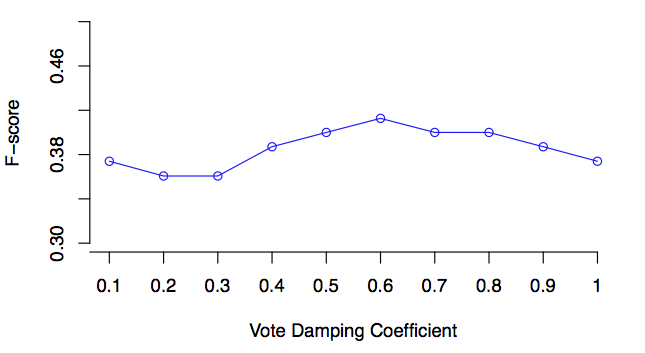
\includegraphics[width=100mm]{graphs/damping.png}
\end{center}
\caption{Effect of damping coefficient on F-score}
\label{fig:damping}
\end{figure}
We use a development set of 100 held-out words from WordNet 1.6 to examine performance while varying various parameters, as described below.
Figure \ref{fig:damping} gives the performance of the algorithm varying the damping coefficient $\gamma$ (described in step \ref{item:voting} of Section \ref{sec:alg}).
The numbers were gathered using scraping for initial enrichment and descriptions for refinement.
Figure \ref{fig:damping} indicates that paying more attention to synsets appearing near the beginning of a word's WordNet entry pays off, but ignoring synsets appearing near the end harms performance, which is entirely expected behavior.
The values collected in Figure \ref{fig:res} use $k=3$ and $\gamma=0.7$, which is close to the optimum of the curve in figure \ref{fig:damping}.

\begin{figure}[htbp]
\begin{center}
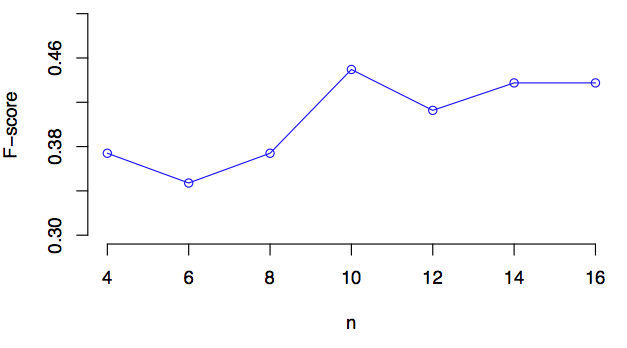
\includegraphics[width=100mm]{graphs/n.png}
\end{center}
\caption{Effect of $n$ on F-score}
\label{fig:n}
\end{figure}
Figure \ref{fig:n} shows the effect varying the value of $n$ has on the F-score.
Recall that $n$ is the number of neighbors of the test word that we take from the offline model in order to reorder them subsequently using a search engine.
We again use scraping for initial enrichment and descriptions for refinement, with $k=3$ and $\gamma=0.7$.

It is not immediately obvious that this curve should decrease past a certain point, but this makes some sense---past a point, the neighbors of the test word are not very semantically related to it, and considering them as members of the eventual set of $k$ neighbors does more harm than good.
Note the values collected in Figure \ref{fig:res} use $n=9$, which is below the optimal value on the curve in Figure \ref{fig:n}, but requires significantly fewer network calls than the optimal $n=22$.

\begin{figure}[htbp]
\begin{center}
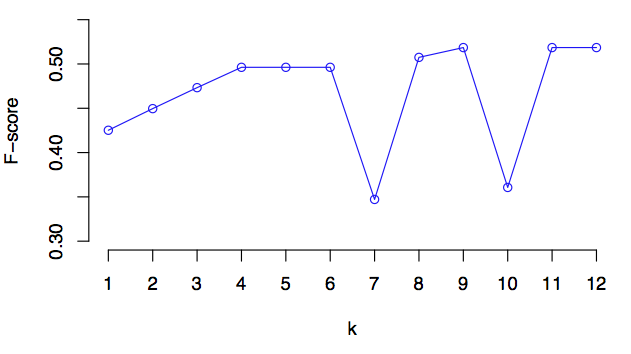
\includegraphics[width=100mm]{graphs/k.png}
\end{center}
\caption{Effect of $k$ on F-score}
\label{fig:k}
\end{figure}
Figure \ref{fig:k} gives the effect of varying $k$, the number of neighbors ultimately used in the voting scheme.
As above, we use scraping for initial enrichment and descriptions for refinement, and we set $n=24$ and $\gamma=0.7$.
It is unclear why this graph is so much less smooth than the others.
The numbers are generated on a relatively small devset of 100 words, so some amount of noise is to be expected in the data.
For the experiments in Figure \ref{fig:res}, we use $k=3$, which is not unreasonable, but $k=4$ or $5$ would likely be preferable.

\begin{figure}[htbp]
\begin{center}
\begin{tabular}{|c|c|c|c||c|c|c|c|}
\hline
  \multicolumn{4}{|c||}{{\bf 1.6 Test Set}} & \multicolumn{4}{c|}{{\bf 1.7 Test Set}}  \\
  {\bf P} & {\bf R} & {\bf A} & {\bf F} & {\bf P} & {\bf R} & {\bf A} & {\bf F} \\
\hline \hline
45.57 & 89.26 & 43.20 & 60.35 & 25.84 & 33.20 & 17.00 & 29.06 \\
\hline
\multicolumn{3}{|c|}{{\it (increase over fig \ref{fig:res}):}} & 6.34 & \multicolumn{3}{c|}{{\it (increase over fig \ref{fig:res}):}}  & x  \\
\hline
\end{tabular}
\caption{Results on 1.6 and 1.7 testsets with tuned params (using enrichment by scraping, refinement by descriptions, $\gamma=0.6$, $k=5$, $n=20$)}
\label{fig:tunedres}
\end{center}
\end{figure}
%We used the results from Figure \ref{fig:res} to determine the experimental setup on which to test these parameter changes.
We  reran one configuration from Figure \ref{fig:res} (Enrichment = ``scrape'', Refinement = ``descriptions''---the setup we used to test the parameter changes) with the optimal values for the parameters.
Figure \ref{fig:tunedres} gives the performance of the configuration with tuned parameters.
Optimizing the values of the parameters improves performance significantly.


\subsection{Discussion}

%Is your hypothesis supported? What conclusions do the results support about the strengths and weaknesses of your method compared to other methods? How can the results be explained in terms of the underlying properties of the algorithm and/or the data.

We hypothesized that using data from the web (for both vector enrichment and refining lists of nearest neighbors) will help performance.
This hypothesis is largely supported by the results given in Figure \ref{fig:res} on the 1.6 test set and refuted by results on the 1.7 test set.

On the 1.6 test set, both types of initial vector enrichment---with descriptions and by scraping pages---outperform the algorithm without enrichment.
Enrichment by descriptions outperforms enrichment by scraping in two of three cases.
In two of three cases, refining with descriptions provides an improvement over no refinement.
Contrary to expectations, in all three cases, refining with scraping harms performance.
By and large, using information from the web on the 1.6 test set helps more than it hurts (with the exception of refining by scraping pages).

On the 1.7 test set, on the other hand, using information from the web harms performance across the board.
The 1.7 test set contains a significantly higher percentage of items with supersense {\it noun.person}---62.60\%, vs 26.11\% in the 1.6 test set.
One unfortunate consequence of this fact is that baseline performance is very difficult to beat on the 1.7 test set (indeed, the baseline outperforms our algorithm in every setup).

Many of the 1.7 test words are proper names of individuals.
These names typically occur quite infrequently in our offline corpus of newswire; therefore, the terms' neighbors in the vector space model are of fairly low quality.
Further, the results from the search engine are often of low quality, in particular because proper names are very much associated with company websites containing those names, and this yields very poor results.
The fact that our algorithm works poorly on proper names is not particularly important for the 1.6 test set, but causes very poor performance on the 1.7 test set, which is comprised of a majority of proper names.
However, performance on the 1.6 test set indicates that givan a more well-balanced set of words, using web data can, in fact, help performance.

One reason we believe that scraped results often hurts performance is the relatively small variety of data collected through this method.
While the hope is that scraping pages allows for a much greater level of contextual information than the limited descriptions from search engine results, we found that this often was the not the case.
First, because scraping websites requires additional network calls, time constraints prevented us from scraping every site the search engine returned---of the approximately 1000 pages typically returned by the search engine, we scraped the top 50 results.
Second, many websites issued 403 Forbidden errors or chose not respond to our request at all due to a systematic ban on scraping.
We believe that changing our crawler's User Agent would have helped this latter issue significantly.

\begin{figure}[hbtp]
\begin{center}
\begin{tabular}{|l|r|r|}
    \hline
    \bf{System} & \bf{WN 1.6} & \bf{WN 1.7}\\
    \hline
    \hline
    Ciaramita and Johnson baseline & 21\% & 28\%\\
    Ciaramita and Johnson perceptron & 53\% & 53\%\\
    Curran similarity-based results & 68\% & 63\%\\
    \hline
    Our baseline & 26\% & 63\%\\
    Our results with optimized parameters & 43\% & 17\%\\
    \hline
\end{tabular}
\caption{Accuracy results compared to Ciaramita \& Johnson, Curran.}
\label{fig:compareresults}
\end{center}
\end{figure}

Figure \ref{fig:compareresults} contains our results compared to those of Ciaramita \& Johnson \cite{cj} and Curran \cite{curran}.
As expected, our impoverished system underperforms both other works in the area.
Since we do not use the same exact test sets or corpora as them, comparative results should be taken with a grain of salt.

One very interesting effect to note is that our 1.7 baseline differs dramatically from the Ciaramita and Johnson baseline. 
Indeed, our 1.7 baseline is as high as Curran's overall accuracy.
Furthermore, Ciaramita \& Johnson report having more difficulty due to the large number of nouns in the $abstract$ category, rather than a large number of proper names as we find.
We believe this is a result of the nature of our corpus---they use a different corpus, and the overlaps between the words added to WordNet 1.7.1 and the different corpora could vary widely.


\section{Related Work}

%Answer the following questions for each piece of related work that addresses the same or a similar problem. What is their problem and method? How is your problem and method different? Why is your problem and method better? 

There are two papers about the particular task of supersense acquisition of nouns.
The first, in which the task is first described, is by Ciaramita \& Johnson \cite{cj}.
They apply a multiclass perceptron classifier which uses a mix of features standardly used in NER, WSD, and lexical disambiguation---parts of speech of neighboring words, $n$-grams in surrounding contexts, and morphological features, for example.
They train on two corpora by, for each unambiguous noun with an entry in WordNet 1.6, calculating a feature vector for each occurrence of that noun.
One corpus is the Bllip corpus, a 40M word corpus of WSJ text; the other is comprised of the definitional glosses collected from WordNet.
The method given in this paper is based entirely on using offline, preprocessed corpora, and augmenting it with results from search engine queries could be fruitful.

The task is approached differently by Curran \cite{curran}.
He uses a more unsupervised approach: construct a distributional vector space model from a large corpus and use a $k$-nearest-neighbors voting scheme to guess the supersense label of an unknown word.
Our basic, offline model is an impoverished version of Curran's---whereas the dimensions in his model correspond to nouns being observed standing in different relations to verbs (e.g. ``being the direct object of {\it give}''), the dimensions in our model correspond simply to nouns being observed within the local contexts of other words.
Our general approach differs from his in that we attempt to also use a search engine---both to augment the initial vector for the unknown word with a greater number of contexts, and also to refine our guess for what the $k$-nearest neighbor vectors are.

Ciaramita and Altun \cite{ciaramita-altun} apply an HMM to the task of WSD on the Supersense level.
That is, instead of guessing supersenses for unknown nouns, they attempt to label individual occurrences of words with appropriate supersenses.
This is a significantly more complicated problem than the one addressed here, and it is not at all obvious how one could use information from the web to help in the task.

%Erk \cite{erk} gives an approach to the somewhat related problem of detecting unknown word senses---automatically detecting occurrences of words in text whose senses are not in a given sense inventory.

The idea of using the web to build models for natural language processing tasks is certainly not novel.
For example, \cite{bollegala} and \cite{gracia} use the results of search engine queries to calculate semantic similarity between terms.
\cite{strube} and \cite{gabrilovich} also use the web to calculate semantic similarity, but restrict themselves to Wikipedia.
However, as far as we know, there is no prior work using the web to guess supersenses of unknown words.
Further, we believe use of search engine queries to refine an initial approximate answer provided by an offline model (in contrast to building a model from the web) is not a widely used technique.
This is the primary contribution of the present work.

\section{Future Work}

%What are the major shortcomings of your current method? For each shortcoming, propose additions or enhancements that would help overcome it. 

One of the primary shortcomings of the current work is the impoverished offline model we use.
As noted above, we chose a simpler vector space model than Curran \cite{curran} and used a much smaller corpus for reasons of time and ease of implementation.
It would be useful to compare Curran's method to the exact same method augmented with refinement using search engine queries; however, this was infeasible for us given the scope of the project.

One of the primary shortcomings of the evaluation we use is the test set---since we use a different test set, comparing our performance directly with prior work is difficult.
For example, we do not lemmatize nouns in our test set, whereas Ciaramita and Johnson \cite{cj} do not indicate if they do or not.
It would be fruitful to obtain the exact training and test sets used in prior work for purposes of comparison.

The general approach we take is to construct a rough first approximation of an answer from a relatively small offline corpus and then use a search engine to refine this approximation.
This approach could be fruitful for a number of different tasks---guessing word similarity or automatically finding synonyms, for example.
Any task whose process of constructing a solution admits refinement with a search engine  could potentially see improvement using this method.

We use the web in two different ways---the first is to enrich the initial query vector for the word with unknown supersense; the second is to refine our guess of what the $k$-nearest neighbors to that vector are.
The manner in which we undertake the latter task is by calculating a set of nearest neighbors of size greater than $k$, reordering these neighbors using information from the web, and taking the $k$-nearest neighbors from this reordered list.
That is, we essentially use information from the web to reorder the list of nearest neighbors.
It remains to be seen if there is a more intelligent way to use the web to  refine our model.
For example, including offline data in the web corpus and allowing new neighboring words to be introduced in the refinement step are both experimental conditions we would wish to explore further.

\section{Conclusion}

%Briefly summarize the important results and conclusions presented in the paper. What are the most important points illustrated by your work? How will your results improve future research and applications in the area? 

We give a method of guessing supersenses of unknown nouns by augmenting a prebuilt offline model with a relatively small number of very targeted search engine queries.
Results are mixed---in particular, testing on words drawn from WordNet 1.6 yields promising results, but the algorithm performs poorly on words new to WordNet 1.7.
However, this certainly does not discredit the potential effectiveness of the general method.

We gather two different types of contexts from the web (using search engine descriptions and scraping the pages ourselves), and try using these contexts in two different ways (in order to enrich our initial representation of the test word and in order to refine our guess about its neighbors).
There may be more ways to use the web than this.
More importantly, the general strategy of using a search engine to refine an approximate offline model (as compared to building a model entirely from web data) is, as far as we know, not particularly widely explored, and could potentially find fruitful applications in different tasks.



\bibliography{writeup}{}
\bibliographystyle{plain}


\end{document}